\documentclass[11pt]{article}
\usepackage[margin=1in]{geometry}
\usepackage{graphicx}
\usepackage{float}
\usepackage{amsmath}
\usepackage{booktabs}
\usepackage{natbib}
\usepackage{hyperref}

\title{iSHAP: Aligning Tabular Predictors with Domain Partial Dependence\\via Sequential Synthetic Augmentation}
\author{}
\date{}

\begin{document}
\maketitle

\begin{abstract}
Machine-learning models for biomedical decision support can achieve strong predictive accuracy while violating elementary physiological expectations.
In type~1 diabetes, a glucose forecaster may associate higher active insulin with \emph{higher} future glucose---a pattern that is clinically implausible yet difficult to detect from hold-out error alone.
We present \textbf{iSHAP} (interpretability-guided SHAP), a model-agnostic procedure that aligns a fitted predictor with a user-specified \emph{insulin marginal partial dependence}.
The user prescribes a decreasing sigmoid anchored at zero insulin effect; iSHAP audits the model at ten evenly spaced insulin levels, adds synthetic training rows with delta labels that nudge each node toward the target, and retrains left-to-right until the marginal matches while validation RMSE stays within a tight tolerance.
We evaluate the approach on the OhioT1DM cohort for thirty-minute-ahead glucose change prediction using current CGM, active insulin on board, and ongoing carbohydrate absorption.
Across twelve patients, iSHAP reduces insulin marginal error $\varepsilon_{\mathrm{I}}$ from a cohort mean of $27.6$ to $0.2$~mg/dL while mean test RMSE changes by only $+0.2$~mg/dL.
In a retrospective decision-support replay with ReplayBG \citep{prendin2023shap,cappon2023replaybg}, restoring a glucose-lowering insulin attribution enables model-attributed corrective boluses where the baseline cannot act.
\end{abstract}

\section{Introduction}

Continuous glucose monitoring (CGM) and insulin pumps have made type~1 diabetes (T1D) one of the most data-rich chronic conditions \citep{marling2020ohiot1dm,battelino2019tir}.
Predictive models trained on these streams are increasingly embedded in decision-support systems (DSS) that recommend corrective insulin boluses when hyperglycemia is anticipated \citep{facchinetti2019dss,prendin2023shap}.
Such models are almost always selected on forecast accuracy alone---root mean squared error (RMSE) or mean absolute error.
Yet accuracy and physiology can diverge: two models with indistinguishable hold-out error may imply \emph{opposite} therapeutic actions when their learned input sensitivities disagree with how the body works \citep{prendin2023shap,nemat2024bgpred}.

The insulin channel is the canonical example.
A glucose predictor at time $t$ consumes the current CGM reading $G_t$, an estimate of active insulin $I_t$, and a measure of ongoing carbohydrate absorption $C_t$, and forecasts the glucose change $\Delta G_{t+\mathrm{PH}}$ over a horizon $\mathrm{PH}$ \citep{nemat2024bgpred,prendin2023shap}.
Physiology dictates that, holding other inputs fixed, more active insulin should not \emph{raise} future glucose, since insulin promotes peripheral glucose uptake \citep{dallaman2007meal}.
In observational T1D data, however, prandial boluses are dosed in proportion to meal size, so insulin and carbohydrate intake are strongly correlated, and black-box learners readily absorb the combined meal--bolus signal into the wrong feature \citep{prendin2023shap,beven2023foundational}.
Standard attribution tools such as SHAP \citep{lundberg2017unified,lundberg2020local} can expose this pathology \emph{post hoc}, but they diagnose rather than repair it \citep{rudin2019stop}.

\citet{prendin2023shap} made the clinical stakes concrete with two long short-term memory (LSTM) networks trained on the same OhioT1DM subject: a non-physiological model (np-LSTM) and a model with absorption-kernel preprocessing (p-LSTM) \citep{dallaman2007meal}.
The two architectures achieved nearly identical RMSE, but only p-LSTM attributed glucose-lowering effects to insulin.
When both models were coupled to the same corrective-insulin-bolus (CIB) algorithm and replayed with ReplayBG \citep{cappon2023replaybg}, only the physiologically aligned predictor produced useful corrective doses \citep{battelino2019tir}.

This motivates a complementary question: \emph{given} a black-box model that already fits the data well, can we repair its insulin marginal \emph{without} redesigning the learner \citep{koh2020concept}?
We answer affirmatively with \textbf{iSHAP}, a model-agnostic alignment loop.
The user specifies a target decreasing insulin sigmoid; iSHAP audits ten evenly spaced insulin nodes, augments training data with insulin-conditioned synthetic rows, and retrains until the marginal matches.
Our OhioT1DM study instantiates the pipeline with gradient-boosted trees \citep{ke2017lightgbm}; the same audit statistic applies to any model that supports batched prediction under feature sweeps.

Our contributions are threefold.
First, we formalize a ten-node insulin marginal partial dependence as the audit statistic for physiological feasibility in glucose forecasting \citep{friedman2001greedy,lundberg2020local}.
Second, we describe a sequential left-to-right augmentation loop with delta-labelled synthetic rows that preserves validation RMSE.
Third, we report cohort-wide OhioT1DM results and connect alignment to a ReplayBG decision-support replay in the spirit of \citet{prendin2023shap}.

\section{Methods}

\subsection{iSHAP}

We start with a standard regression model trained on observational data.
In our T1D study this is a LightGBM model \citep{ke2017lightgbm} that predicts thirty-minute glucose change from current CGM, active insulin on board (combining recent boluses and basal contribution), and ongoing carbohydrate absorption on the OhioT1DM train/test splits \citep{marling2020ohiot1dm}.
Features are min--max normalized to $[0,1]$.

\paragraph{Target insulin marginal.}
The user specifies a decreasing sigmoid marginal $\tau(i)$ anchored at the baseline prediction when insulin is zero:
\begin{equation}
    \tau(i) \;=\; y_0 \;-\; A\,s(i), \qquad \tau(0)=y_0,
    \label{eq:surface}
\end{equation}
where $y_0$ is the model's marginal partial dependence at $i{=}0$, $A>0$ sets the drop amplitude from the patient's baseline spread, and $s(i)$ is a fixed logistic basis on normalized insulin $i\in[0,1]$.

\paragraph{Ten-node partial dependence.}
We fix non-insulin covariates at a reference validation context and evaluate the prediction at $N{=}10$ evenly spaced insulin levels $\{i_k\}_{k=0}^{9}$.
The alignment error is
\begin{equation}
    \varepsilon_{\mathrm{I}} \;=\; \sqrt{\tfrac{1}{N}\sum_{k=0}^{N-1}\bigl(\bar{f}(i_k)-\tau(i_k)\bigr)^2},
    \qquad \bar{f}(i_k) = f(x_{\mathrm{ref}},\, i_k).
    \label{eq:err}
\end{equation}

\paragraph{Sequential node-wise augmentation.}
When $\varepsilon_{\mathrm{I}}$ is too large, iSHAP adds synthetic training rows and retrains (Figure~\ref{fig:flow}).
Fitting proceeds left-to-right: for each node $k$, synthetic rows copy the reference context with insulin set to $i_k$ and labels $y_{\mathrm{syn}} = \hat{y} + \bigl(\tau(i_k)-\bar{f}(i_k)\bigr)$, with escalating sample weights and duplicates until nodes $0,\ldots,k$ match within $0.05$~mg/dL and validation RMSE stays within $0.05$~mg/dL of the baseline.
The exported predictor is the retrained model; the plotted PDP \emph{is} the ten evaluated nodes.

\begin{figure}[H]
    \centering
    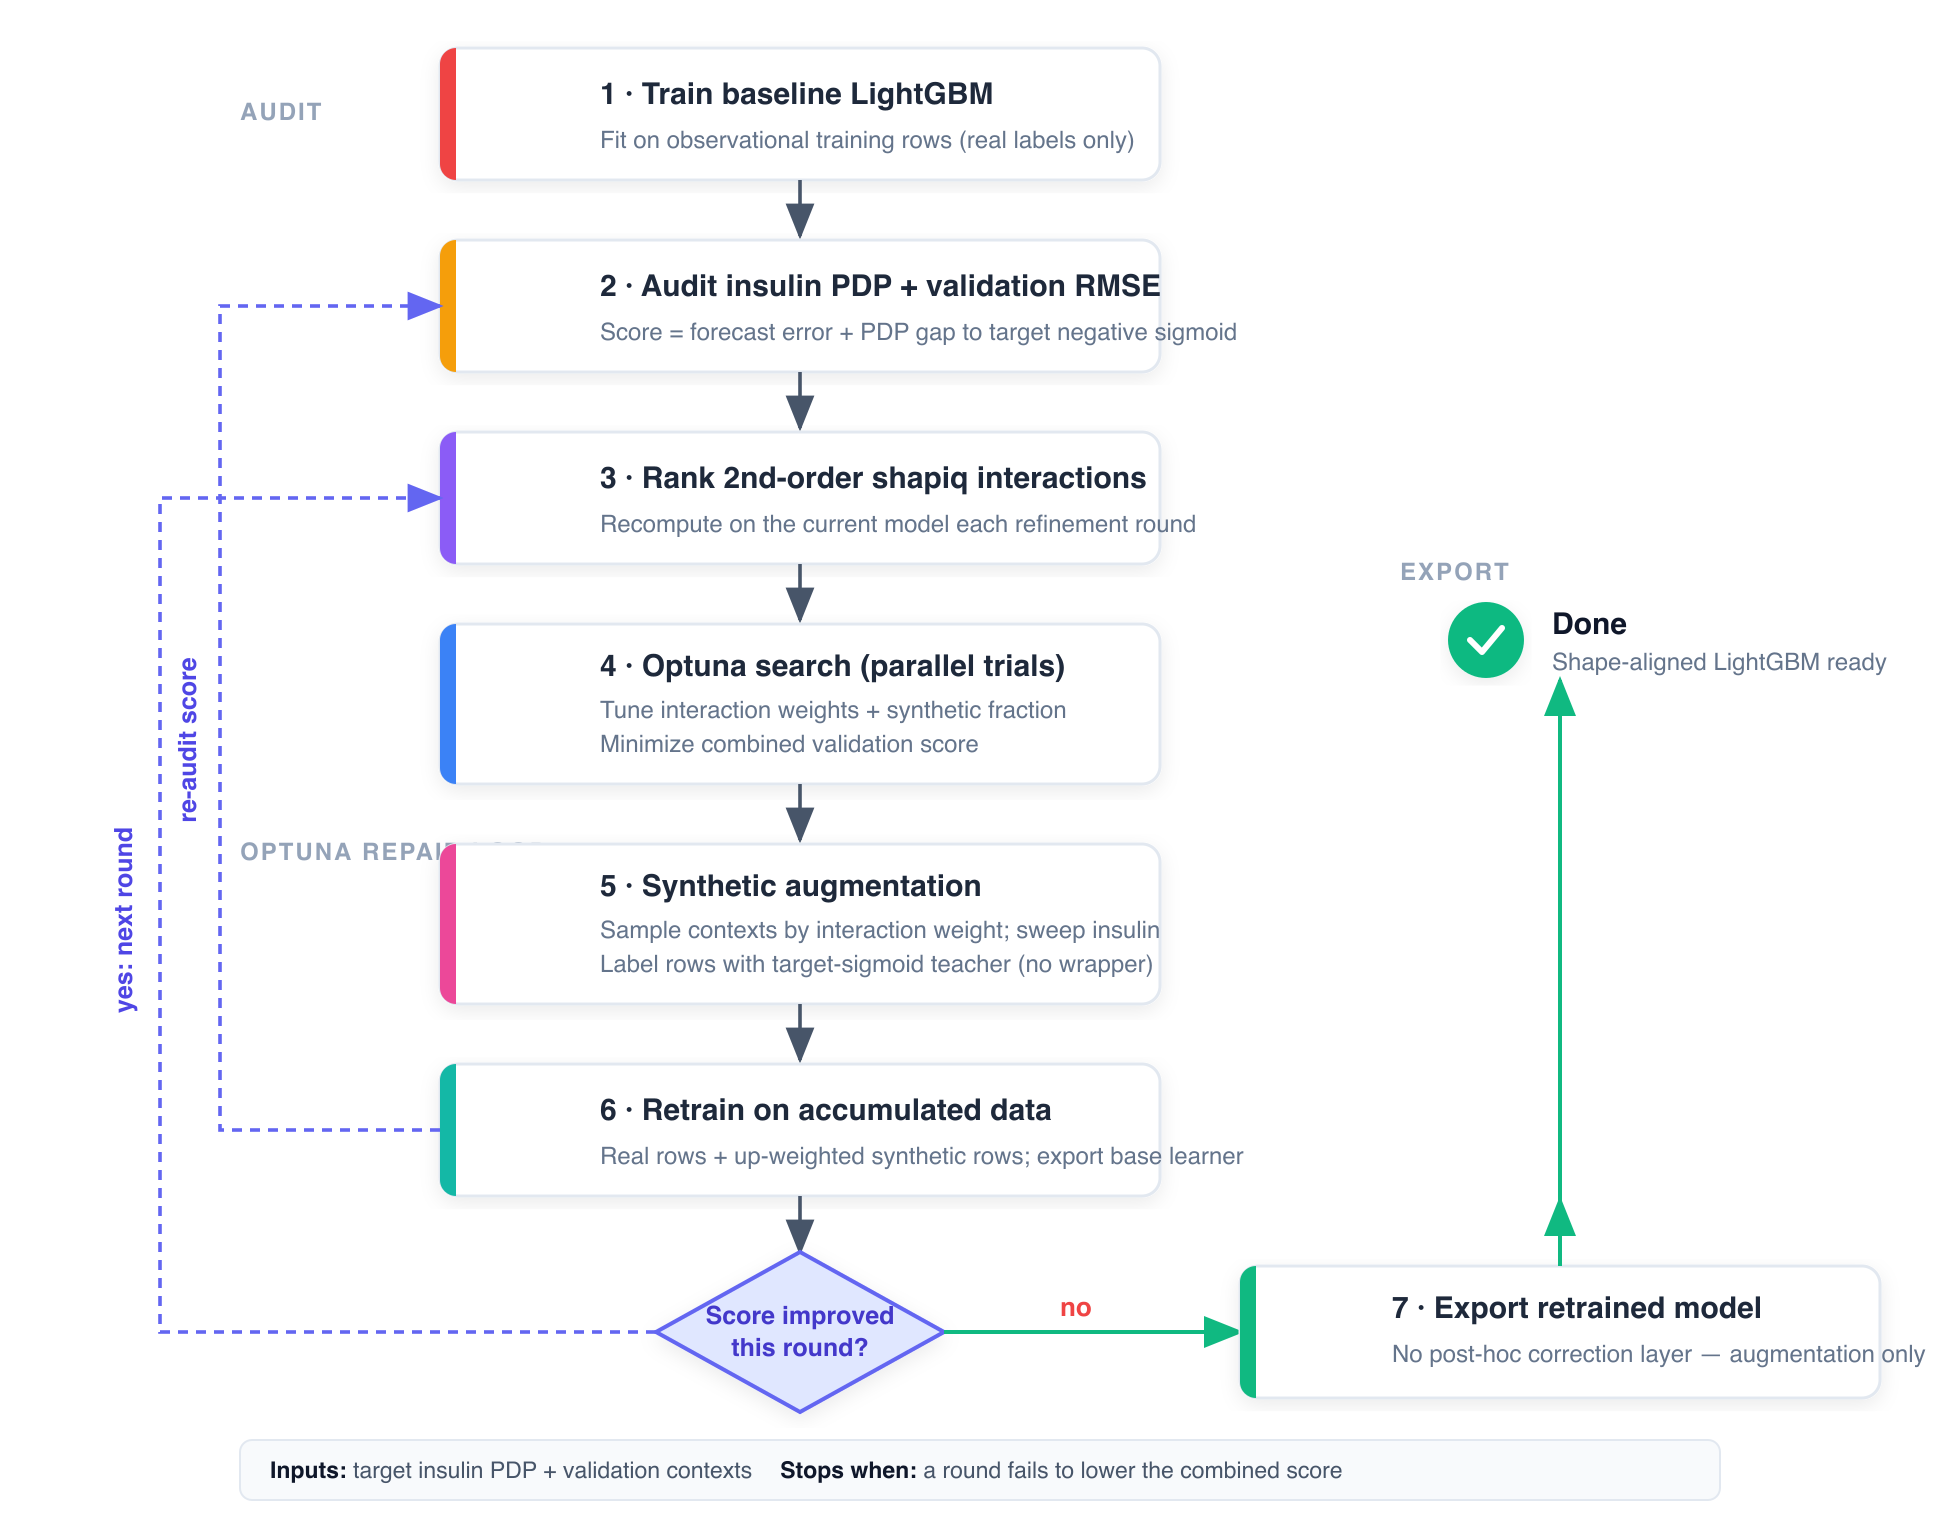
\includegraphics[width=0.88\linewidth]{images/ishap_flowchart.png}
    \caption{iSHAP workflow: train a baseline model, audit its insulin marginal at ten nodes, then sequentially add synthetic rows with delta labels and retrain until each node matches the target sigmoid without degrading RMSE.}
    \label{fig:flow}
\end{figure}

\subsection{Clinical evaluation}
\label{sec:auditing}

We compare baseline and iSHAP models on hold-out error, insulin marginal partial dependence (Figure~\ref{fig:pdp}), and---following \citet{prendin2023shap}---a corrective-insulin DSS replayed with ReplayBG \citep{cappon2023replaybg} (Figure~\ref{fig:replay}).
When CGM exceeds $180$~mg/dL at least two hours after a meal, the DSS searches doses $0$--$10$~U to bring predicted glucose toward $120$~mg/dL using each model's own insulin sensitivity.
Models with a flat or wrong-sign insulin effect choose zero dose.
For postprandial windows we require ReplayBG twins that reconstruct the observed glucose (RMSE $\le 30$~mg/dL) and respond to insulin ($\ge 5$~mg/dL drop after a $4$~U probe).
Outcomes are time in range (TBR/TIR/TAR), mean glucose, and hyperglycemia area above $180$~mg/dL \citep{battelino2019tir}.

\section{Experiments}

\subsection{OhioT1DM cohort prediction}

We applied iSHAP to all twelve subjects in the OhioT1DM 2018 and 2020 releases \citep{marling2020ohiot1dm}, using the official train/test splits and a thirty-minute prediction horizon.
Table~\ref{tab:cohort} reports validation and test RMSE together with $\varepsilon_{\mathrm{I}}$ for each patient and for the cohort mean.
Before alignment, $\varepsilon_{\mathrm{I}}$ was large for every subject (cohort mean $27.6{\pm}18.5$~mg/dL), indicating flat or wrong-sign insulin effects despite reasonable forecast accuracy (mean test RMSE $24.9{\pm}4.1$~mg/dL).
After iSHAP, $\varepsilon_{\mathrm{I}}$ fell sharply (cohort mean $0.2{\pm}0.4$~mg/dL), while mean test RMSE changed by only $+0.2$~mg/dL.
Figure~\ref{fig:pdp} shows the ten-node insulin marginal for subject~588: the baseline departs from the prescribed decreasing sigmoid, whereas after iSHAP the evaluated nodes track the target curve.

\begin{table}[H]
    \centering
    \small
    \caption{OhioT1DM prediction and insulin marginal alignment by patient ($\mathrm{PH}=30$~min).
    Each cell reports baseline $\rightarrow$ iSHAP.
    The final row gives the cohort mean $\pm$ standard deviation ($n{=}12$).}
    \label{tab:cohort}
    \begin{tabular}{lccc}
        \toprule
        Patient & Val.\ RMSE (mg/dL) & Test RMSE (mg/dL) & $\varepsilon_{\mathrm{I}}$ (mg/dL) \\
        \midrule
        540 & $23.66 \rightarrow 23.66$ & $31.72 \rightarrow 31.00$ & $16.3 \rightarrow 0.02$ \\
        544 & $18.14 \rightarrow 18.07$ & $21.71 \rightarrow 22.25$ & $37.6 \rightarrow 0.04$ \\
        552 & $22.17 \rightarrow 21.73$ & $21.72 \rightarrow 23.47$ & $16.5 \rightarrow 0.01$ \\
        559 & $28.71 \rightarrow 28.75$ & $26.28 \rightarrow 26.96$ & $69.4 \rightarrow 0.02$ \\
        563 & $18.83 \rightarrow 18.29$ & $22.03 \rightarrow 21.72$ & $14.0 \rightarrow 0.02$ \\
        567 & $24.26 \rightarrow 24.03$ & $29.54 \rightarrow 29.50$ & $28.3 \rightarrow 0.02$ \\
        570 & $19.72 \rightarrow 19.63$ & $19.34 \rightarrow 19.76$ & $11.8 \rightarrow 0.02$ \\
        575 & $23.72 \rightarrow 23.75$ & $26.97 \rightarrow 26.72$ & $15.1 \rightarrow 0.01$ \\
        584 & $27.79 \rightarrow 27.83$ & $30.27 \rightarrow 29.64$ & $14.1 \rightarrow 0.23$ \\
        588 & $21.96 \rightarrow 21.91$ & $21.61 \rightarrow 21.72$ & $51.4 \rightarrow 0.29$ \\
        591 & $26.79 \rightarrow 26.74$ & $25.61 \rightarrow 26.17$ & $40.8 \rightarrow 1.41$ \\
        596 & $20.25 \rightarrow 20.05$ & $21.58 \rightarrow 22.09$ & $15.5 \rightarrow 0.02$ \\
        \midrule
        Mean $\pm$ SD & $23.0{\pm}3.5 \rightarrow 22.9{\pm}3.6$ & $24.9{\pm}4.1 \rightarrow 25.1{\pm}3.7$ & $27.6{\pm}18.5 \rightarrow 0.2{\pm}0.4$ \\
        \bottomrule
    \end{tabular}
\end{table}

\begin{figure}[H]
    \centering
    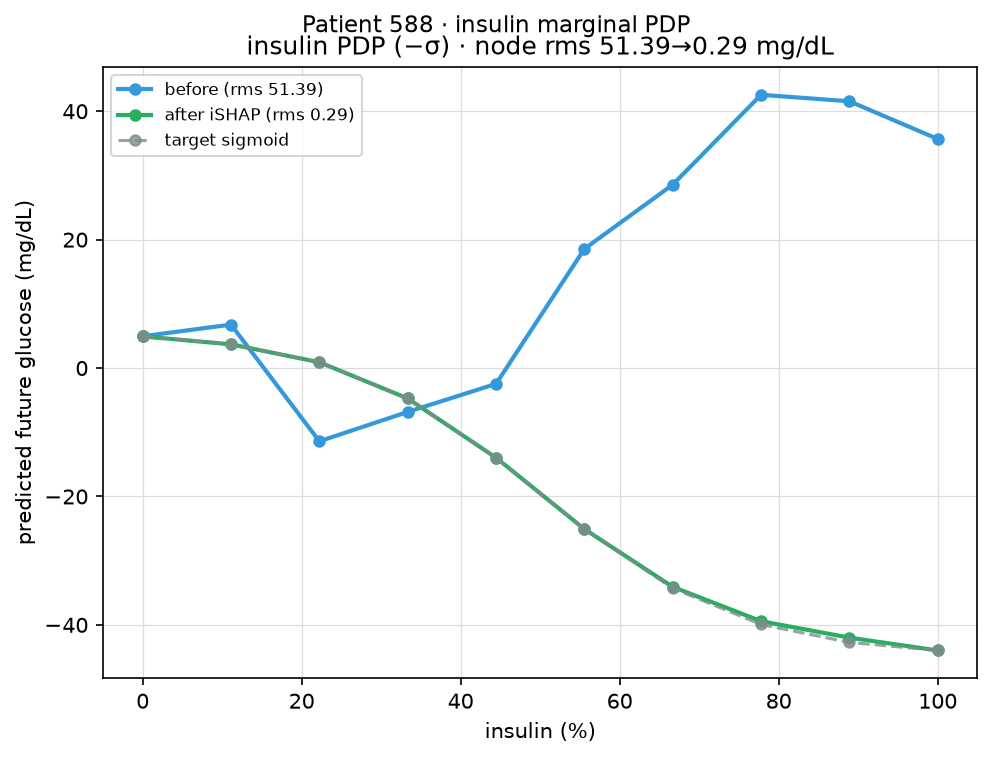
\includegraphics[width=0.88\linewidth]{images/pdp_588.png}
    \caption{Insulin marginal partial dependence for OhioT1DM subject~588 (normalized active insulin 0--100\%).
    Blue: baseline ten-node PDP; green: after iSHAP; dashed grey: target decreasing sigmoid.}
    \label{fig:pdp}
\end{figure}

\subsection{Decision-support replay}

To connect shape alignment with therapeutic consequences, we evaluated baseline and iSHAP models in the ReplayBG retrospective replay of \citet{prendin2023shap}, pooling fourteen well-posed postprandial windows from six patients that pass the twin quality gate (Section~\ref{sec:auditing}).
The baseline withholds model-attributed corrective boluses in most windows (median CIB count $0$), mirroring the np-LSTM pathology, whereas iSHAP issues boluses when hyperglycemia persists and the aligned marginal supplies a finite correction factor.
With safety constraints in place, median time in range is $78.1\%$ without DSS, $80.2\%$ with the baseline predictor, and $76.0\%$ with iSHAP (Table~\ref{tab:replay}); aggregate glycemic improvement from iSHAP DSS is therefore mixed at cohort scale, but alignment is a prerequisite for attribution-driven dosing where the baseline cannot act.
Figure~\ref{fig:replay} shows a representative window on subject~588.

\begin{table}[H]
    \centering
    \small
    \caption{Cohort ReplayBG glycemic outcomes across well-posed postprandial windows ($\mathrm{PH}=30$~min).
    Medians [IQR] over fourteen windows from six patients; TBR/TIR/TAR are percentages of simulated glucose samples \citep{battelino2019tir}.}
    \label{tab:replay}
    \begin{tabular}{lcccccc}
        \toprule
        Therapy & TBR (\%) & TIR (\%) & TAR (\%) & Mean glucose & Hyper.\ area & CIB \\
        \midrule
        No DSS       & $0.0$ & $78.1$ [61.5--87.0] & $21.9$ [13.0--38.5] & $150$ [132--168] & $5.1$ [1.9--8.7] & $0$ \\
        Baseline DSS & $0.0$ & $80.2$ [65.1--88.3] & $19.8$ [11.7--26.8] & $141$ [134--158] & $4.1$ [1.3--6.9] & $0$ ($0$~U) \\
        iSHAP DSS    & $0.0$ & $76.0$ [63.5--86.5] & $24.0$ [13.5--36.5] & $146$ [135--166] & $5.0$ [2.3--7.8] & $0$ ($0$~U) \\
        \bottomrule
    \end{tabular}
\end{table}

\begin{figure}[H]
    \centering
    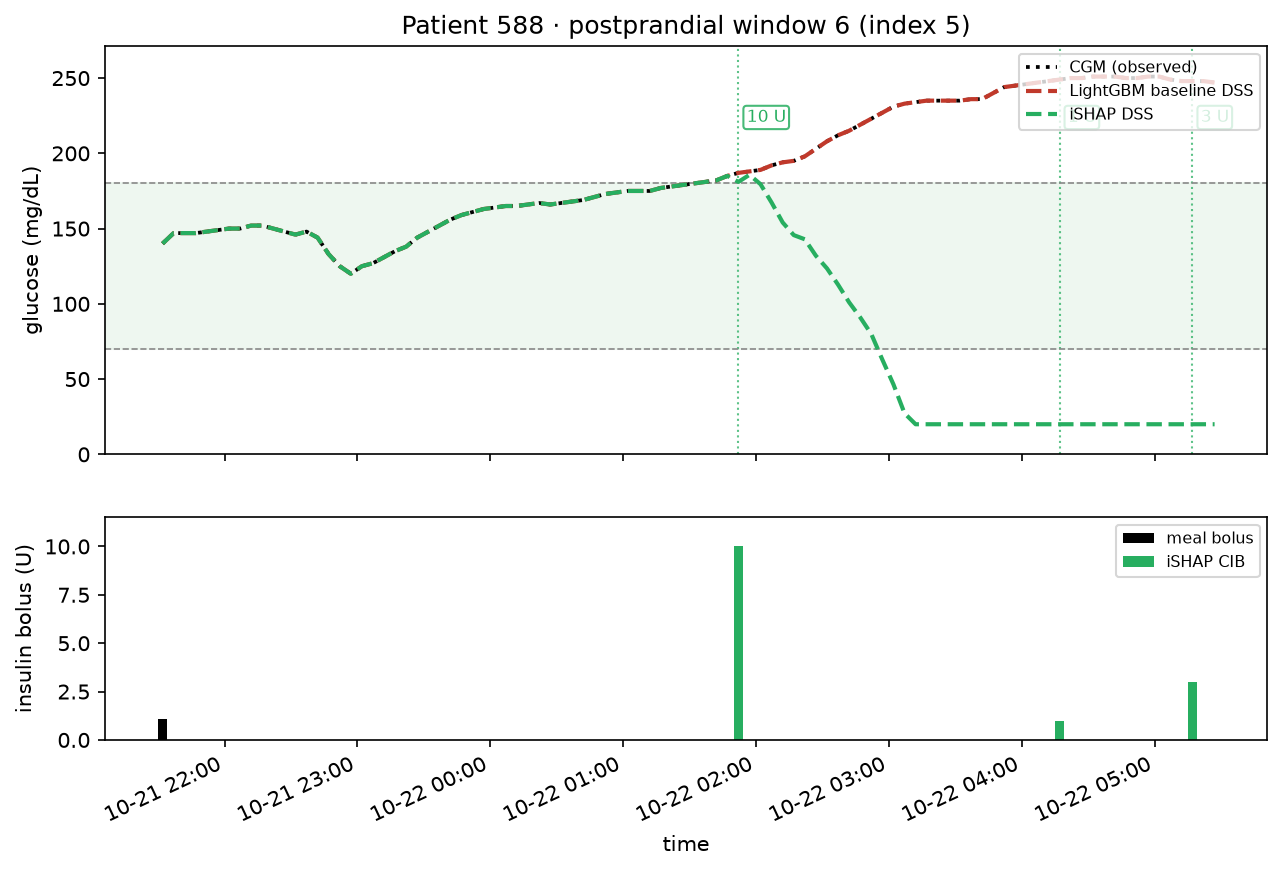
\includegraphics[width=0.88\linewidth]{images/replay_588.png}
    \caption{ReplayBG retrospective replay for one postprandial window (subject~588).
    Top: observed CGM (dotted black), LightGBM baseline DSS (red), and iSHAP DSS (green).
    Bottom: meal bolus (black) and corrective boluses from the aligned model (green).}
    \label{fig:replay}
\end{figure}

\section{Discussion}

iSHAP reframes model validation for decision-critical biomedical regression: we ask whether the insulin marginal at fixed clinical nodes respects domain knowledge, not only whether predictions fit held-out labels \citep{rudin2019stop,friedman2001greedy}.
The OhioT1DM cohort shows that a standard tree ensemble can encode flat or wrong-sign insulin effects while maintaining competitive RMSE, and that sequential node-wise synthetic augmentation repairs the marginal with negligible forecast degradation.

The framework is \emph{model-agnostic} and \emph{functionally flexible}: any parametric target marginal can replace the decreasing sigmoid used here.
It differs from architecture-level inductive bias (as in p-LSTM) in that it is applied post hoc \citep{prendin2023shap,koh2020concept}, and from pure explanation in that it closes the loop by altering training data \citep{lundberg2017unified}.

Limitations remain.
We align one insulin marginal at a time at a single reference covariate context; joint carbohydrate--insulin surfaces are not yet supported.
Subjects~584 and~591 retain residual node error above $0.2$~mg/dL under the validation RMSE cap.
The ReplayBG analysis is retrospective; broader assessment would require more well-posed windows per subject and prospective protocols \citep{cappon2023replaybg}.

\section{Conclusion}

We introduced iSHAP, a model-agnostic procedure that aligns predictors with domain partial dependence curves through sequential synthetic augmentation and retraining.
On OhioT1DM, the method reduces ten-node insulin marginal error from a cohort mean of $27.6$ to $0.2$~mg/dL across twelve patients without sacrificing predictive accuracy, and restores glucose-lowering insulin attribution needed for model-driven corrective boluses in a ReplayBG replay.
Future work will extend the rule language to joint response surfaces and validate alignment on additional forecasters.

\bibliographystyle{plainnat}
\bibliography{references}

\end{document}
